\section{Experimental Evaluation}

\subsection{Frozen Protocol and Metric Semantics}
The static experiment uses a fixed five-node heterogeneous fog pool so that increasing $N$ changes offered load rather than infrastructure composition. It tests $N\in\{120,150,180,200,250,300\}$ with 30 paired seeds per scale. Greedy, GA-Hybrid, LPRelax, DPP, MPC, and M-CA-ALM receive the same task, node, and channel realization for each seed. The primary table is a fixed-configuration comparison: GA-Hybrid uses population 100 and 100 generations, whereas M-CA-ALM uses population 50, 50 generations, one ALM step per generation, and repair-aware scoring. This is not an equal search-budget claim. A separate five-seed-per-scale control uses population 100 and 100 generations for both evolutionary methods, with identical environments and final repair; it is reported as a budget-sensitivity control and is not pooled with the 30-seed primary table.

Satisfaction is binary: a task is satisfied only if it is admitted, deadline-timely, and free of resource violation. A dropped task is a deadline and composite violation. Under these definitions, composite violation equals $100$ minus satisfaction and is not reported as an independent improvement. All returned schedules have zero resource violation after shared repair. The run, not the task, is the statistical unit.

The static data comprise 1,080 run-level observations ($6$ loads $\times 6$ methods $\times 30$ paired seeds); the ablation data are reported separately. The reproducibility materials include the MATLAB configuration and SHA-256 hashes of the metric, environment, repair, post-optimization, and solver files. We use two-sided paired sign-flip tests with 20,000 resamples, Holm correction within each comparison family, 95\% confidence intervals for paired differences, and paired Cohen's $d_z$.

\subsection{Static Satisfaction}
Table~\ref{tab:official_static} reports the confirmed means. Light-load cases are saturated and should not be interpreted as algorithmic wins. Separation appears only after $N=120$.

\begin{table*}[t]
\centering
\caption{Official static satisfaction results (30 paired seeds per scale). Differences are M-CA-ALM minus GA-Hybrid in percentage points.}
\label{tab:official_static}
\small
\setlength{\tabcolsep}{3.5pt}
\begin{tabular}{rrrrrrrr}
\toprule
$N$ & Greedy & GA-Hybrid & M-CA-ALM & Paired diff. & 95\% CI & $d_z$ & Holm $p$ \\
\midrule
120 & 62.53 & 83.83 & 89.11 & 5.28 & [2.99, 7.57] & 0.82 & $<0.001$ \\
150 & 24.38 & 39.02 & 40.11 & 1.09 & [0.72, 1.46] & 1.04 & $<0.001$ \\
180 & 21.59 & 37.20 & 37.93 & 0.72 & [0.26, 1.18] & 0.56 & $<0.001$ \\
200 & 21.25 & 33.45 & 36.00 & 2.55 & [1.19, 3.91] & 0.67 & $<0.001$ \\
250 & 21.77 & 30.96 & 34.71 & 3.75 & [2.93, 4.56] & 1.65 & $<0.001$ \\
300 & 22.44 & 27.42 & 31.38 & 3.96 & [3.16, 4.75] & 1.78 & $<0.001$
 \\
\bottomrule
\end{tabular}
\end{table*}

Figure~\ref{fig:static_baselines} is generated directly from archived
run-level and paired-summary files. It visualizes the same six load levels and
six methods as the static tables; the bands are stored 95\% intervals and do
not represent additional experimental runs.

\begin{figure*}[t]
\centering
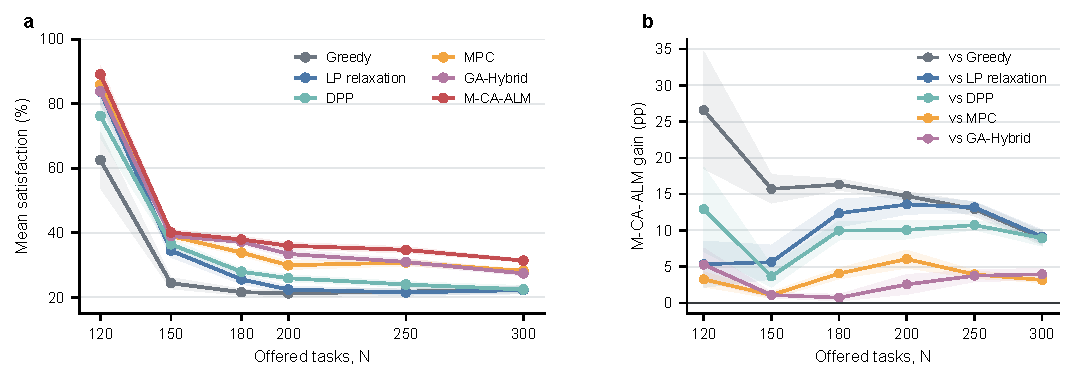
\includegraphics[width=\textwidth]{Fig_Static_Baseline_Comparison.pdf}
\caption{Static baseline comparison.
(a) Mean satisfaction and stored 95\% intervals across 30 paired seeds at
each offered-load level. (b) M-CA-ALM paired satisfaction gain and stored
95\% interval against each implemented baseline. The figure reports only the
fixed five-node simulator and the six tested load levels.}
\label{fig:static_baselines}
\end{figure*}

M-CA-ALM never loses to GA-Hybrid on a paired seed in the six congested scales. Win/tie counts are 28/2 at $N=120$, 25/5 at $N=150$, 14/16 at $N=180$, 24/6 at $N=200$, 28/2 at $N=250$, and 29/1 at $N=300$. The strongest practical effects occur at $N=250$ and $300$, where the paired effect sizes exceed 1.6.

\subsection{Factorial Mechanism Ablation}
We isolate guarded local acceptance ($G$) and repair-aware phenotype ranking ($R$) in a paired $2\times2$ design. Raw disables both factors; Guard enables only $G$; Repair-aware enables only $R$; Full enables both. The four variants use identical environments, solver random streams, final repair, and post-optimization. As an additional reproducibility gate, all 180 Full rows exactly reproduce the corresponding M-CA-ALM rows in the main experiment.

\begin{table}[t]
\centering
\caption{Mean satisfaction (\%) in the 30-seed mechanism ablation.}
\label{tab:official_ablation}
\small
\begin{tabular}{rrrrr}
\toprule
$N$ & Raw & Guard & Repair-aware & Full \\
\midrule
120 & 83.06 & 83.06 & 89.11 & 89.11 \\
150 & 39.69 & 39.69 & 40.11 & 40.11 \\
180 & 36.28 & 36.28 & 37.93 & 37.93 \\
200 & 33.52 & 33.52 & 36.00 & 36.00 \\
250 & 30.65 & 30.65 & 34.71 & 34.71 \\
300 & 27.44 & 27.44 & 31.38 & 31.38 \\
\bottomrule
\end{tabular}
\end{table}

Table~\ref{tab:official_ablation} attributes the observed gain to repair-aware ranking. Its paired main effect ranges from 0.42 to 6.06 percentage points. Full exceeds Raw after Holm correction at five of six scales; $N=150$ is not significant after correcting all ablation comparisons. Guard and Raw are identical on every run, as are Full and Repair-aware, so the estimated guard main effect and interaction are both zero. The guard is therefore a safety invariant in this implementation, not an empirically supported source of higher satisfaction.

\subsection{Cross-Algorithm Transfer and Offline Learned Baseline}
We next test whether repair-aware ranking transfers beyond the ALM search. On independent runs 31--50, GA-Hybrid-Raw and GA-Hybrid-RepairAware use identical environments, evolutionary budgets, random streams, final repair, and post-optimization; only candidate ranking changes. For each run, the paired effect is averaged equally over the six congested scales before inference. Repair-aware GA improves satisfaction by 3.08 points (95\% CI [2.62, 3.68], $d_z=2.48$), wins all 20 run-level pairs, and remains significant after Holm correction. Its scale-wise gain is positive and corrected-significant at every tested $N$, ranging from 1.10 to 4.88 points. The corresponding independent ALM effect is 3.28 points (95\% CI [2.50, 4.40]). This experiment supports repair-aware ranking as an optimizer-independent selection principle within the two tested evolutionary families; it does not establish transfer to arbitrary repair operators.

The learned comparator is a 24-unit bipartite graph policy trained only on runs 51--55, selected only on runs 61--63, and frozen before testing on runs 1--30. The train, selection, and test partitions are disjoint; no test environment updates network parameters or contributes labels. OfflineGNN receives the same final repair, post-optimization, metric code, and paired environments as M-CA-ALM. Its mean satisfaction over $N=120,150,180,200,250,300$ is 74.00\%, 36.27\%, 28.54\%, 26.40\%, 23.80\%, and 22.20\%, respectively. M-CA-ALM is higher at every scale and by 9.67 points after equal scale averaging (95\% CI [8.67, 10.76], $d_z=3.27$; 30/30 run-level wins). Table~\ref{tab:transfer_learning} summarizes the primary paired tests. OfflineGNN is a leakage-free internally trained comparator, not a published method, a new contribution, or a claim of superiority over all learned schedulers.

\begin{table*}[t]
\centering
\caption{Primary paired repair-transfer and offline-learning tests. Effects are satisfaction differences in percentage points after equal averaging over the six congested scales.}
\label{tab:transfer_learning}
\scriptsize
\setlength{\tabcolsep}{2.5pt}
\begin{tabular}{lrrrrrrr}
\toprule
Comparison & Runs & Scales & Mean diff. & 95\% CI & $d_z$ & W/T/L & $p$ \\
\midrule
GA repair-aware $-$ raw & 20 & 6 & 3.08 & [2.62, 3.68] & 2.48 & 20/0/0 & $<0.001$ \\
ALM repair-aware $-$ raw & 20 & 6 & 3.28 & [2.50, 4.40] & 1.41 & 20/0/0 & $<0.001$ \\
M-CA-ALM $-$ OfflineGNN & 30 & 6 & 9.67 & [8.67, 10.76] & 3.27 & 30/0/0 & $<0.001$ \\
\bottomrule
\end{tabular}
\end{table*}

\subsection{Additional Mathematical and Control Baselines}
We add three non-learning comparator baselines under the same final repair and evaluation protocol: an admission-aware LP relaxation with deterministic rounding (LPRelax), a deadline-ordered dynamic placement heuristic (DPP), and a short-horizon rollout controller (MPC). The LP solves a linear memory/load proxy and is not treated as an exact optimum for the nonlinear simulator. Table~\ref{tab:official_baselines} reports the mean satisfaction for all six compared methods at the congested scales.

\begin{table*}[t]
\centering
\caption{Mean satisfaction (\%) with additional static baselines (30 paired seeds per scale).}
\label{tab:official_baselines}
\small
\begin{tabular}{rrrrrrr}
\toprule
$N$ & Greedy & GA-Hybrid & LPRelax & DPP & MPC & M-CA-ALM \\
\midrule
120 & 62.53 & 83.83 & 83.78 & 76.19 & 85.86 & 89.11 \\
150 & 24.38 & 39.02 & 34.49 & 36.44 & 39.02 & 40.11 \\
180 & 21.59 & 37.20 & 25.56 & 27.94 & 33.87 & 37.93 \\
200 & 21.25 & 33.45 & 22.42 & 25.93 & 29.95 & 36.00 \\
250 & 21.77 & 30.96 & 21.52 & 23.97 & 30.77 & 34.71 \\
300 & 22.44 & 27.42 & 22.26 & 22.44 & 28.21 & 31.38
 \\
\bottomrule
\end{tabular}
\end{table*}

M-CA-ALM is higher than every comparator on every scale in the paired means. The five paired comparisons at each scale remain significant after Holm correction over all 30 ALM-versus-baseline tests; the largest adjusted value is $0.0015$. MPC is the strongest low-cost competitor at high load, but remains 3.17 percentage points below M-CA-ALM at $N=300$ while running roughly 50 times faster. This comparison exposes the practical trade-off rather than hiding it: the proposed method buys satisfaction with second-scale computation, whereas MPC is preferable when latency budget dominates.

\subsection{Admission and Runtime Trade-off}
Admission is 100\% through $N=200$. At $N=250$, mean admission is 93.25\% for M-CA-ALM and 93.28\% for GA-Hybrid; at $N=300$, it is 86.94\% and 86.89\%, respectively. Satisfaction gains therefore do not come from materially more aggressive admission.

M-CA-ALM is consistently slower. Its mean runtime is 3.10--3.18 times that of GA-Hybrid, increasing from 0.50~s at $N=120$ to 1.11~s at $N=300$. GA-Hybrid increases from 0.16~s to 0.35~s. This cost is compatible with the measured second-scale simulation windows, but it is not evidence for millisecond scheduling or deployment latency.

The equal-budget control changes the interpretation of the primary comparison. At $N=120,150,180,200,300$, the ALM--GA-Hybrid paired mean differences are $-4.00$, $-1.07$, $-0.67$, $+0.10$, and $-0.07$ percentage points, respectively; at $N=250$ the difference is $+2.32$ points. The five-run control is therefore mixed rather than uniformly favorable to M-CA-ALM. Its ALM runtime is approximately 3.4--4.3 times the GA-Hybrid runtime. These results prevent the fixed-configuration advantage from being attributed solely to a method advantage under equal computation; the supported claim is that repair-aware ALM can be effective in the tested congested regime, with substantial computation cost and load-dependent outcome.

\subsection{State-Preserving Replay and the Overload Boundary}
We next embed Greedy, GA-Hybrid, and M-CA-ALM in a separate 500-slot state-preserving replay at $N\in\{180,300\}$. Each scale uses 20 paired environment runs. Unresolved tasks retain their identities across slots, the backlog is capped at $N$, and all methods observe the same arrivals and environment seed in each paired run. This replay is a dynamic experiment with carry-over state and repeated arrivals, not a temporal extension of the one-shot static experiment; its observations are therefore analyzed separately. The replay contains 60,000 slot records and 120 run records. Before analysis, validation checks duplicate keys, complete slot coverage, algorithm pairing, seed matching, and resource feasibility.

\begin{table}[t]
\centering
\caption{State-preserving 500-slot replay results (20 paired runs per scale). Saturation is the first slot with backlog equal to its cap.}
\label{tab:official_replay}
\scriptsize
\begin{tabular}{llrrr}
\toprule
$N$ & Method & Mean sat. & Median full slot & Queue drops \\
\midrule
180 & Greedy & 28.70 & 3 & 38,280 \\
180 & GA-Hybrid & 33.45 & 7 & 30,486 \\
180 & M-CA-ALM & \textbf{46.41} & \textbf{56} & \textbf{24,550} \\
300 & Greedy & 3.78 & 2 & 138,535 \\
300 & GA-Hybrid & \textbf{8.97} & 2 & \textbf{122,994} \\
300 & M-CA-ALM & 3.51 & 2 & 139,345 \\
\bottomrule
\end{tabular}
\end{table}

At $N=180$, M-CA-ALM exceeds GA-Hybrid by 12.96 percentage points in mean satisfaction (95\% CI [5.79, 20.12], $d_z=0.79$), wins all 20 paired runs, and remains significant after Holm correction ($p=0.00080$). Its median first full-backlog slot is 56, compared with 7 for GA-Hybrid and 3 for Greedy; one ALM run never reaches the cap. Thus, the dynamic benefit is expressed not only in slot satisfaction but also in delayed queue saturation and fewer queue-cap drops.

The $N=300$ replay defines a different operating regime. Every method reaches the backlog cap at slot 2 in every run. M-CA-ALM averages 3.51\% satisfaction, compared with 8.97\% for GA-Hybrid and 3.78\% for Greedy. The ALM--GA difference is negative, but does not remain significant after family-wise Holm correction ($p=0.152$). We therefore treat $N=300$ as an immediate-overload boundary, not as evidence of dynamic superiority. Figure~\ref{fig:replay_overload} shows how this boundary changes both cumulative completions and queue-cap losses.

\begin{figure*}[t]
\centering
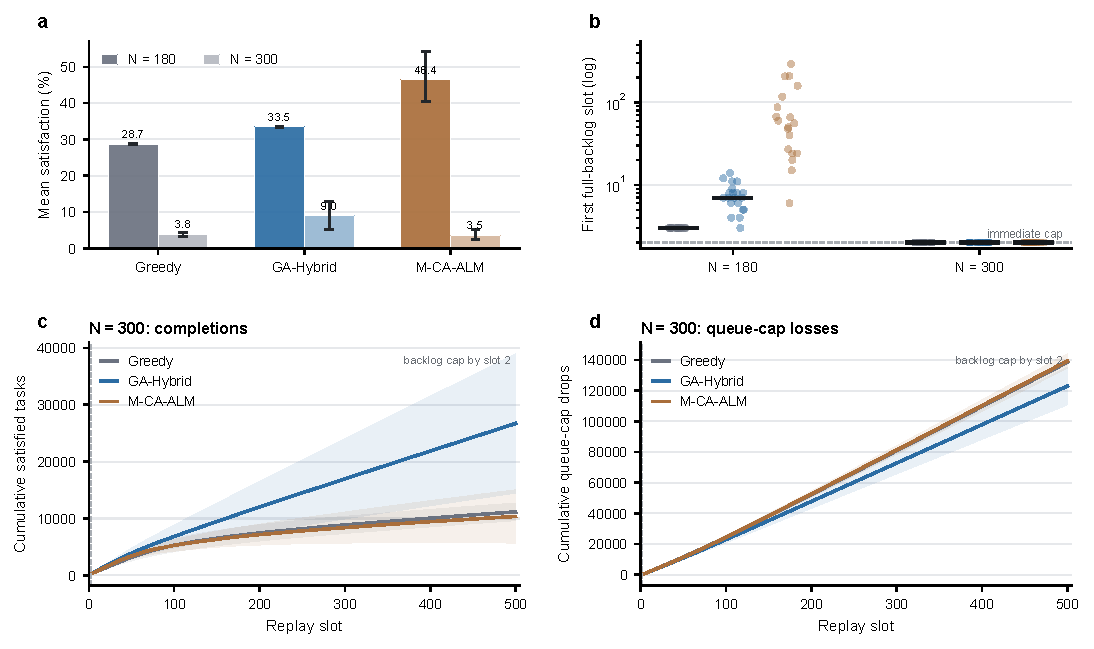
\includegraphics[width=\textwidth]{Fig_Replay_Overload_Boundary.pdf}
\caption{Static-to-dynamic operating boundary. (a) Mean slot satisfaction with run-level 95\% confidence intervals. (b) First full-backlog slot for each paired run; black lines indicate medians and the vertical axis is logarithmic. (c) Cumulative satisfied tasks at $N=300$. (d) Cumulative queue-cap drops at $N=300$. Bands in (c)--(d) are 95\% confidence intervals over 20 runs. At $N=300$, all methods reach the backlog cap at slot 2, so the result bounds rather than extends the recoverable-congestion claim.}
\label{fig:replay_overload}
\end{figure*}
